% fig_method.tex -- Figure 1: the method in pictures (TikZ, drawn by hand; absolute coordinates in cm, natural width about 18.7 cm).
%   (a) test time: the image goes through the frozen U-Net up to block A (the pass stops there); of every block ONE number is read (the
%       amplitude: per channel the largest deviation from the spatial mean, log, mean over channels).  The numbers form the profile.  The
%       score is one Mahalanobis distance: from the profile to the point mu*.
%   (b) once, before: the n held-out ID images in the eight orientations of the square.  As they are: mean mu and covariance S of the
%       profile.  The seven other orientations: the mean mu_o.  No feature of a training image is stored.
%   (c) what the score means: mu* is mu moved away from mu_o; a profile on the mu_o side is far from mu*.
%   Colours: black, navy (ID side), red (the test image / what is computed).  The curves and the layout of (c) are a schematic, not data.
\begin{tikzpicture}[font=\scriptsize, >={Stealth[length=1.5mm, width=1.2mm]}, line join=round, line cap=round,
  lab/.style={font=\tiny, inner sep=1pt, align=center}, ttl/.style={font=\scriptsize, anchor=south west, inner sep=0pt}]
\def\unet#1#2#3#4#5{% origin (left block, centre height), scale, style of the down path and bottom, style of block A, style of the rest of the up path
  \begin{scope}[shift={#1}, scale=#2]
    \foreach \dx/\yc/\h in {0/0/1.5, 0.3/0/1.5, 0.75/-0.5/1.0, 1.05/-0.5/1.0, 1.5/-0.95/0.6, 1.8/-0.95/0.6, 2.25/-0.95/0.6, 2.55/-0.95/0.6}
      \draw[#3] (\dx,\yc-\h/2) rectangle ++(0.22,\h);
    \draw[#4] (3.2,-1.0) rectangle ++(0.22,1.0);
    \foreach \dx/\yc/\h in {3.5/-0.5/1.0, 3.95/0/1.5, 4.25/0/1.5}
      \draw[#5] (\dx,\yc-\h/2) rectangle ++(0.22,\h);
    \draw[#3] (0.52,0) -- (0.75,-0.5) (1.27,-0.5) -- (1.5,-0.95) (2.02,-0.95) -- (2.25,-0.95) (2.77,-0.95) -- (3.2,-0.5);
    \draw[#5] (3.72,-0.5) -- (3.95,0);
  \end{scope}}
%% ================================================================ (a) test time
\node[ttl] at (0,0.3) {\textbf{(a)}\ テスト時：ブロックAまで通し,ブロックごとに数値を1つだけ読む};
\node[inner sep=0, draw=black!60] at (0.62,-1.0) {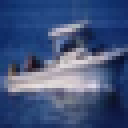
\includegraphics[width=1.0cm]{figs/ex_id.png}};
\node[lab, anchor=north] at (0.62,-1.57) {テスト画像 $\vec{x}$};
\draw[->] (1.16,-1.0) -- node[above, lab] {$+\sigma_1\veps$} (1.84,-1.0);
\unet{(1.9,-1.0)}{1}{black, line width=0.7pt}{redc, fill=redc!35, line width=0.9pt}{black!40, densely dashed, line width=0.5pt}
\node[lab, anchor=south west] at (1.9,-0.2) {ノイズ除去器(U-Net, 凍結). 順伝播は1回};
\node[lab, anchor=north west, text=redc] at (5.02,-2.03) {\textbf{ブロックA}で止める};
\draw[black!70, decorate, decoration={brace, mirror, amplitude=3pt}] (1.9,-2.42) -- (5.32,-2.42);
\node[lab, anchor=north] at (3.6,-2.55) {ブロックAまでの出力};
% ---- the amplitude of one block: one channel, the largest deviation from its spatial mean
\draw[->] (6.5,-1.0) -- (7.2,-1.0);
\foreach \i/\j/\s in {0/0/12,1/0/20,2/0/8,3/0/15,4/0/10, 0/1/18,1/1/10,2/1/25,3/1/12,4/1/8, 0/2/8,1/2/15,2/2/12,3/2/90,4/2/20, 0/3/14,1/3/8,2/3/18,3/3/22,4/3/10, 0/4/10,1/4/16,2/4/9,3/4/13,4/4/17}
  \fill[black!\s] ({7.3+0.26*\i},{-0.55-0.26*\j}) rectangle ++(0.26,-0.26);
\draw[black!60] (7.3,-0.55) rectangle (8.6,-1.85);
\draw[redc, line width=1.0pt] (8.08,-1.07) rectangle ++(0.26,-0.26);
\node[lab, anchor=south] at (7.95,-0.52) {ブロック $h$ の1チャネル};
\node[lab, anchor=north, text=redc] at (7.95,-1.88) {平均から最も離れた値};
\node[lab, anchor=north] at (7.95,-2.2) {その大きさの対数を\\チャネルで平均};
\draw[->] (8.7,-1.2) -- node[above, lab] {$a_h(\vec{x})$} node[below, lab] {数値1つ} (9.75,-1.2);
% ---- the profile: one number per block up to A
\draw[black!45, rounded corners=3pt] (9.8,-0.2) rectangle (14.25,-3.15);
\draw[->, black!80] (10.25,-2.8) -- (14.1,-2.8); \draw[->, black!80] (10.25,-2.8) -- (10.25,-0.4);
\node[lab, anchor=north east] at (14.15,-2.84) {ブロック $h$};
\node[lab, anchor=south west] at (10.3,-0.62) {振幅 $a_h$};
\fill[navyc!18] (10.5,-1.75) -- (11.0,-1.45) -- (11.5,-1.6) -- (12.0,-1.25) -- (12.5,-1.0) -- (13.0,-1.35) -- (13.5,-1.15) -- (13.95,-1.45)
  -- (13.95,-1.95) -- (13.5,-1.65) -- (13.0,-1.85) -- (12.5,-1.5) -- (12.0,-1.75) -- (11.5,-2.1) -- (11.0,-1.95) -- (10.5,-2.25) -- cycle;
\draw[navyc, line width=0.9pt] (10.5,-2.0) -- (11.0,-1.7) -- (11.5,-1.85) -- (12.0,-1.5) -- (12.5,-1.25) -- (13.0,-1.6) -- (13.5,-1.4) -- (13.95,-1.7);
\draw[black, densely dashed, line width=0.8pt] (10.5,-1.75) -- (11.0,-1.4) -- (11.5,-1.5) -- (12.0,-1.05) -- (12.5,-0.75) -- (13.0,-1.15) -- (13.5,-0.9) -- (13.95,-1.15);
\draw[redc, line width=1.0pt] (10.5,-2.2) -- (11.0,-2.05) -- (11.5,-2.4) -- (12.0,-2.0) -- (12.5,-2.1) -- (13.0,-1.95) -- (13.5,-2.25) -- (13.95,-2.3);
\foreach \p in {(10.5,-2.2),(11.0,-2.05),(11.5,-2.4),(12.0,-2.0),(12.5,-2.1),(13.0,-1.95),(13.5,-2.25),(13.95,-2.3)} \fill[redc] \p circle (0.05);
\node[lab, anchor=south, text=redc] at (13.95,-0.75) {A};
\draw[black!55, densely dotted] (13.95,-2.8) -- (13.95,-0.78);
\node[lab, anchor=west] at (10.42,-0.95) {$\vmu^{*}$(破線)};
\node[lab, anchor=west, text=navyc] at (11.75,-0.62) {分布内の画像($\vmu$ と幅)};
\node[lab, anchor=west, text=redc] at (10.42,-2.62) {テスト画像 $\va(\vec{x})$};
\draw[<->, redc, line width=0.5pt] (12.5,-0.8) -- (12.5,-2.05);
% ---- one distance -> the score
\draw[->] (14.35,-1.6) -- (14.85,-1.6);
\node[draw=black, rounded corners=2pt, line width=0.9pt, inner sep=3pt, align=center, font=\tiny, text width=20mm] at (16.1,-1.6) {$\vmu^{*}$ までの\\マハラノビス距離\\(式は1つ)};
\draw[->] (17.3,-1.6) -- (17.75,-1.6);
\node[lab, anchor=west] at (17.72,-1.6) {$s(\vec{x})$};
\node[lab, anchor=north, text=black!60] at (16.1,-2.3) {近いほど分布内};
%% ================================================================ (b) prepared once
\node[ttl] at (0,-3.95) {\textbf{(b)}\ 事前の準備(1回だけ)：分布内の画像\olNRefMax{}枚を8つの向きで通す};
\node[inner sep=0, draw=navyc, line width=0.8pt] at (0.5,-5.0) {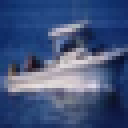
\includegraphics[width=0.62cm]{figs/ex_id.png}};
\node[lab, anchor=north, text=navyc] at (0.5,-5.36) {そのまま};
\foreach \x/\y/\r/\sx/\sy in {1.55/-4.72/0/1/-1, 2.3/-4.72/0/-1/1, 3.05/-4.72/180/1/1, 3.8/-4.72/90/1/1, 1.55/-5.52/270/1/1, 2.3/-5.52/90/1/-1, 3.05/-5.52/270/1/-1}
  \node[inner sep=0, rotate=\r, xscale=\sx, yscale=\sy] at (\x,\y) {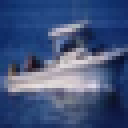
\includegraphics[width=0.62cm]{figs/ex_id.png}};
\node[lab, anchor=west] at (3.45,-5.52) {残り7つの向き};
\draw[->] (4.7,-5.1) -- (5.15,-5.1);
\unet{(5.25,-4.95)}{0.3}{black, line width=0.35pt}{redc, fill=redc!35, line width=0.35pt}{black!40, densely dashed, line width=0.3pt}
\draw[->] (6.7,-5.1) -- (7.15,-5.1);
\pgfmathsetseed{7}
\foreach \i in {1,...,12} {\pgfmathsetmacro{\sa}{0.2*(rnd-0.5)}\pgfmathsetmacro{\sb}{0.2*(rnd-0.5)}\pgfmathsetmacro{\sc}{0.2*(rnd-0.5)}\pgfmathsetmacro{\sd}{0.2*(rnd-0.5)}\pgfmathsetmacro{\se}{0.2*(rnd-0.5)}
  \draw[navyc!55, line width=0.3pt] (7.3,{-4.85+\sa}) -- (7.7,{-4.55+\sb}) -- (8.1,{-4.7+\sc}) -- (8.5,{-4.3+\sd}) -- (8.9,{-4.5+\se});}
\foreach \i in {1,...,12} {\pgfmathsetmacro{\sa}{0.2*(rnd-0.5)}\pgfmathsetmacro{\sb}{0.2*(rnd-0.5)}\pgfmathsetmacro{\sc}{0.2*(rnd-0.5)}\pgfmathsetmacro{\sd}{0.2*(rnd-0.5)}\pgfmathsetmacro{\se}{0.2*(rnd-0.5)}
  \draw[black!45, line width=0.3pt] (7.3,{-5.75+\sa}) -- (7.7,{-5.6+\sb}) -- (8.1,{-5.85+\sc}) -- (8.5,{-5.6+\sd}) -- (8.9,{-5.8+\se});}
\draw[->, navyc, line width=0.9pt] (9.1,-4.6) -- (9.6,-4.6);
\node[lab, anchor=west, text=navyc] at (9.62,-4.6) {平均 $\vmu$,共分散 $\Sm$};
\draw[->, black!70, line width=0.9pt] (9.1,-5.7) -- (9.6,-5.7);
\node[lab, anchor=west] at (9.62,-5.7) {平均 $\vmu_{o}$};
\node[lab, anchor=west] at (0.1,-6.35) {保存するのは $\vmu^{*}$ と $(\Sm+\lambda\bar{s}\Id)^{-1}$ の計\olNStored{}個の数値(CIFAR-10). 勾配による学習も,学習画像の特徴の保存もない};
%% ================================================================ (c) what the score means
\node[ttl] at (12.2,-3.95) {\textbf{(c)}\ スコアの意味};
\draw[black!45, rounded corners=3pt] (12.2,-4.15) rectangle (18.7,-6.55);
\draw[black!55, fill=black!10, rotate around={25:(13.35,-5.85)}] (13.35,-5.85) ellipse (0.62 and 0.3);
\draw[navyc, fill=navyc!18, rotate around={25:(15.0,-5.2)}] (15.0,-5.2) ellipse (0.62 and 0.3);
\foreach \a/\b in {1.25/0.6, 2.05/0.98} \draw[redc!70, densely dashed, line width=0.4pt, rotate around={25:(17.2,-4.33)}] (17.2,-4.33) ++(180:\a) arc[start angle=180, end angle=290, x radius=\a, y radius=\b];
\draw[black!70, line width=0.5pt] (13.35,-5.85) -- (15.0,-5.2);
\draw[->, redc, line width=0.8pt] (15.0,-5.2) -- (17.13,-4.36);
\fill[black!70] (13.35,-5.85) circle (0.05); \fill[navyc] (15.0,-5.2) circle (0.05); \fill[redc] (17.2,-4.33) circle (0.06);
\node[lab, anchor=north] at (13.35,-6.18) {向きを変えた画像};
\node[lab, anchor=south east] at (13.3,-5.8) {$\vmu_{o}$};
\node[lab, anchor=west, text=navyc] at (15.62,-5.38) {分布内の画像};
\node[lab, anchor=south east, text=navyc] at (15.0,-5.15) {$\vmu$};
\node[lab, anchor=west, text=redc] at (17.27,-4.33) {$\vmu^{*}$};
\node[lab, anchor=south east, text=redc] at (16.25,-4.62) {$c(\vmu-\vmu_{o})$};
\fill[redc] (14.35,-6.05) circle (0.045); \draw[redc, line width=0.4pt, densely dotted] (14.35,-6.05) -- (17.2,-4.33);
\node[lab, anchor=west, text=redc] at (14.45,-6.2) {テスト画像のプロファイル};
\node[lab, anchor=east, text=black!60] at (18.6,-6.3) {破線：スコアが等しい線};
\end{tikzpicture}
